\section{Feedback Stimulation Setup} \label{Maxxx}

To elicit electrotactile stimulation in this project, the MaxSens stimulation device will be used along with a 16 multi-pad electrode. The following section will provide a short overview of the stimulation device and multi-pad electrode specifications. 
 

\subsection{Stimulation Electrode}

The 1$\times$16 multi-pad stimulation electrode, can be seen in \figref{fig:electrode}. It is made of 16 circular cathodes, which each share a common long anode. The electrode consists of a polyester layer, an Ag/AgCl conductive layer and a insulation coating. The electrode to skin contact can be improved by applying conductive hydrogel pads to the electrode pads. \cite{Strbac2016}     

\begin{figure}[H]                 
	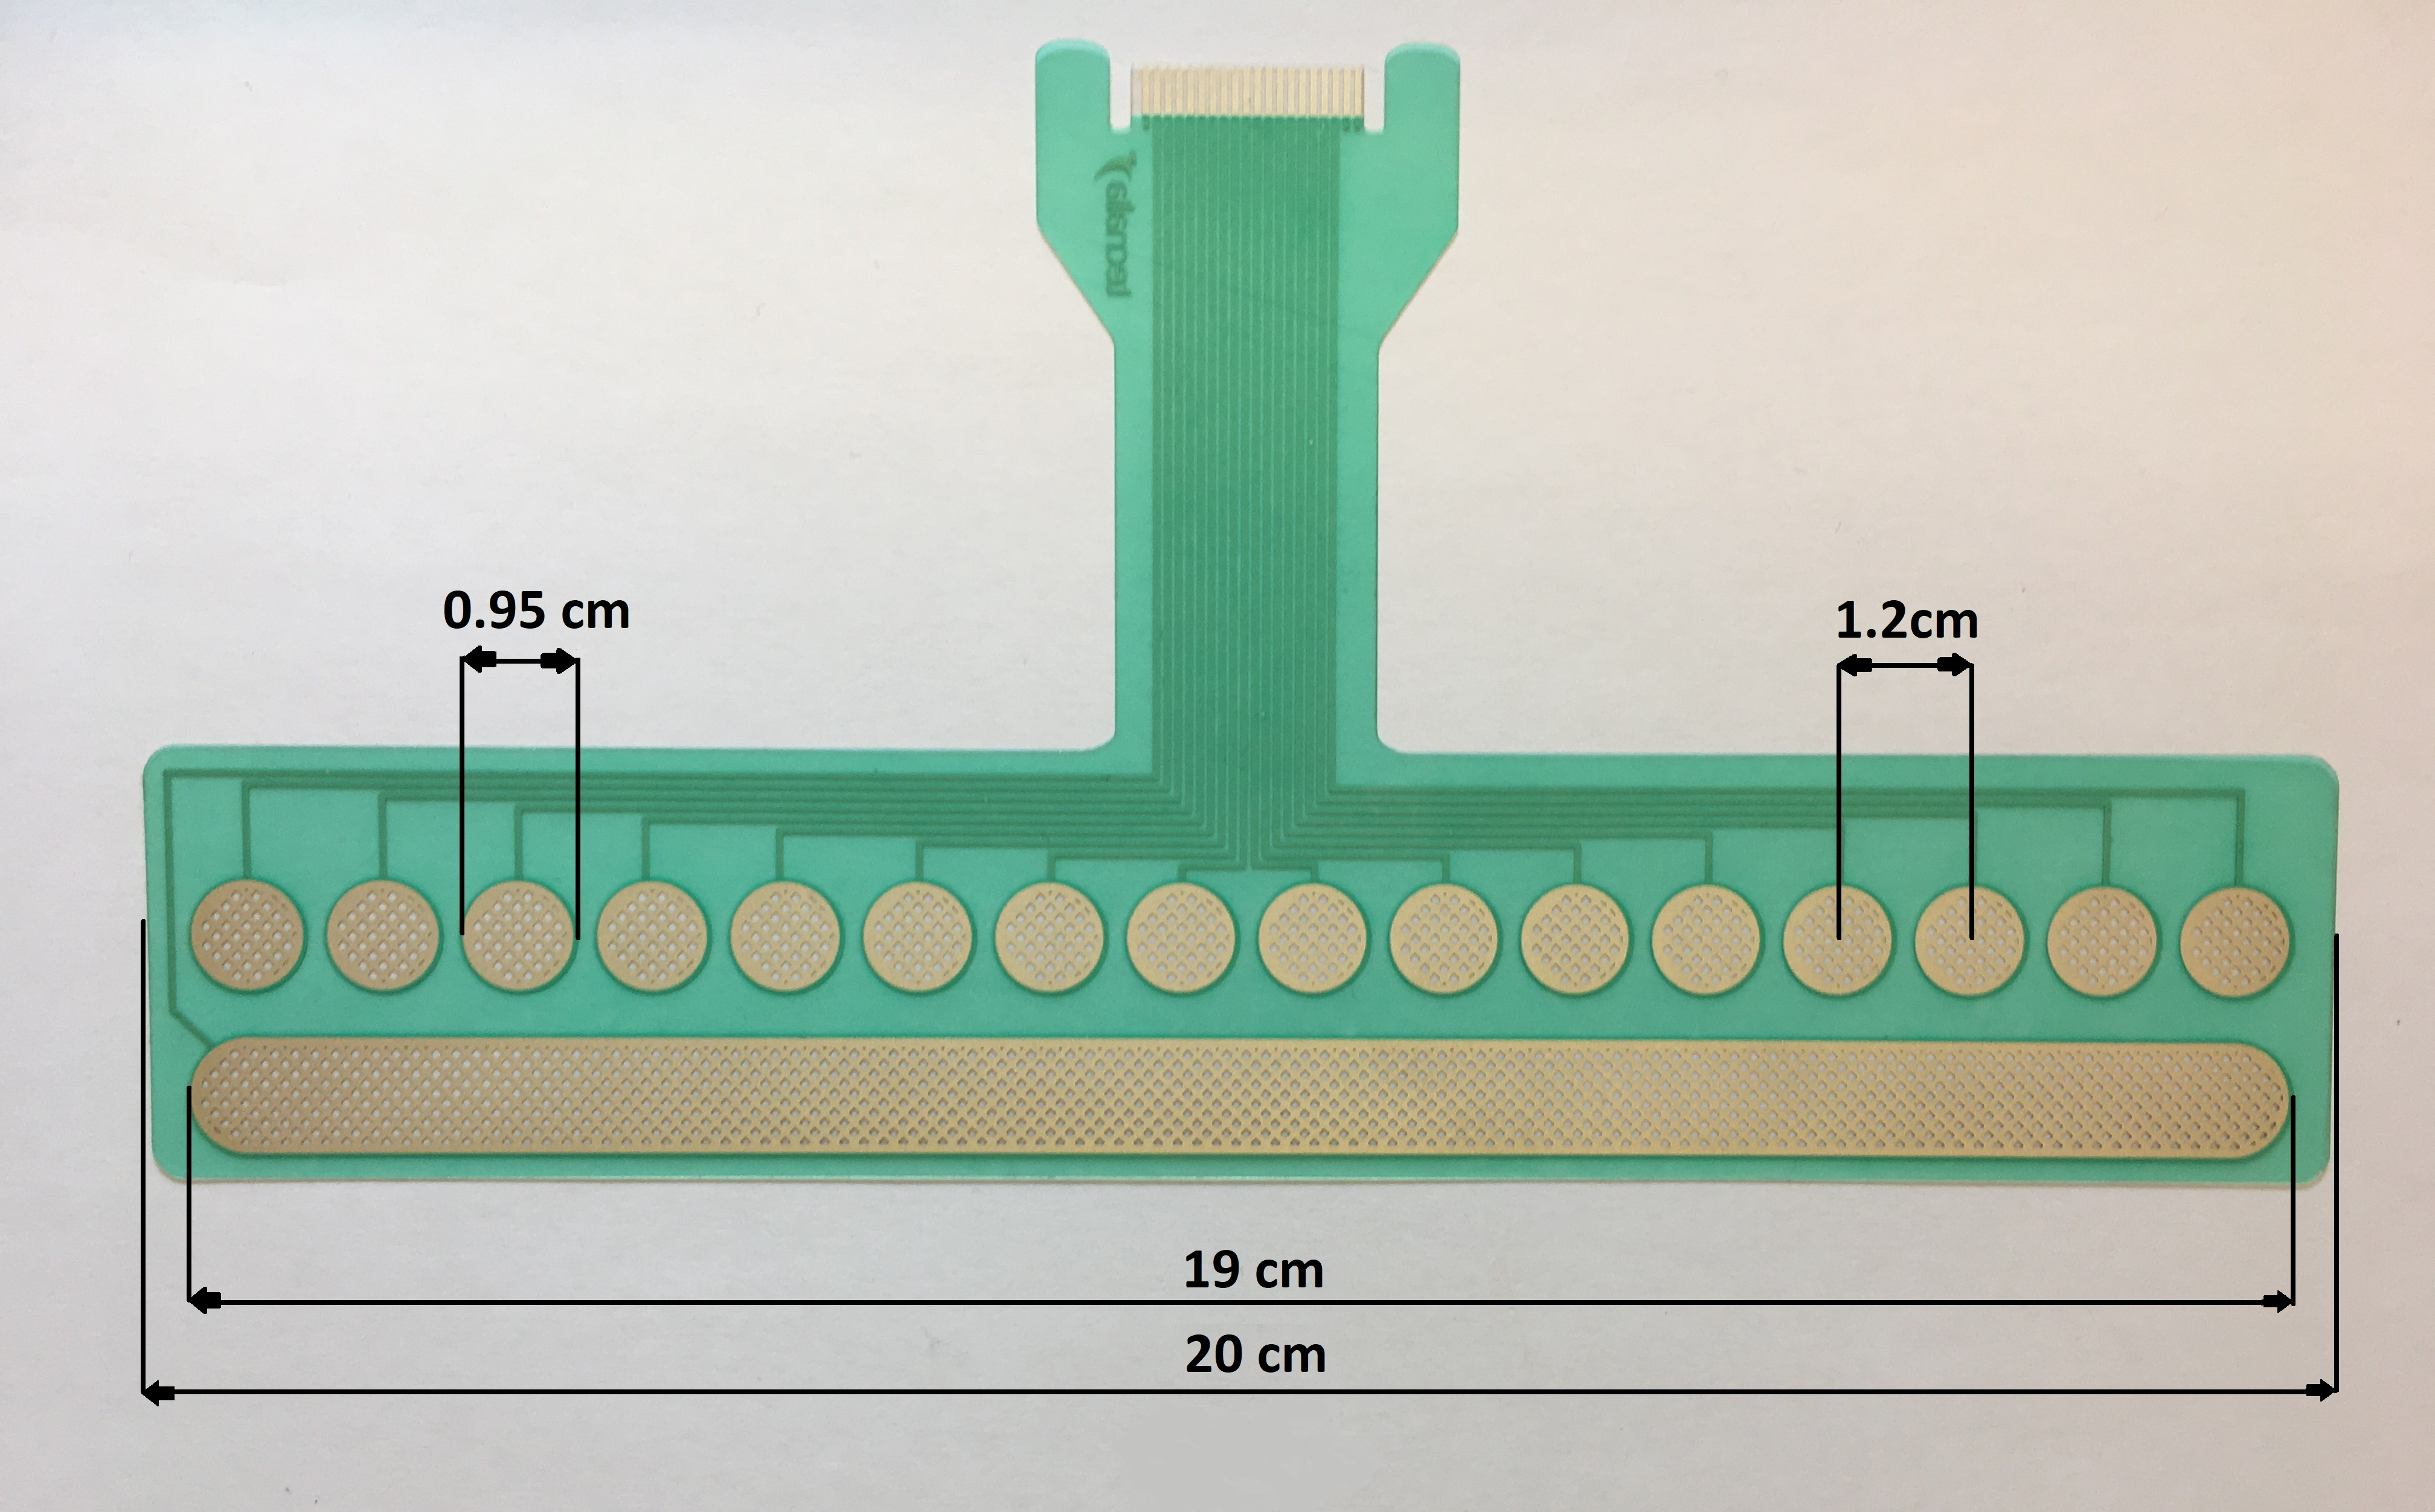
\includegraphics[width=.57\textwidth]{figures/electrode}  
	\caption{The 16 multi-pad electrode used for stimulation consists of 16 circular cathode pads, which each share a common anode.}
	\label{fig:electrode} 
\end{figure}

\subsection{MaxSens Stimulation Device}

The stimulation device is made by MaxSens, Tecnalia, San Sebastian, Spain. Communication between PC and the stimulation device can be achieved either through Bluetooth or USB serial connection. The MaxSens device allows for independent control of the 16 pads in the electrode. It generates biphasic stimulation pulses where the pulse width can be controlled within a 50 - 1000 $\mu $s range with 10 $\mu $s steps, frequency ranges from 1 - 400 Hz with 1 Hz steps and current amplitude ranges from 50 - 10000 $\mu $A with 0.1 $\mu $A steps. Whereas current amplitude and pulse width can be controlled independently for each pad, the pad frequency is set globally limiting all pads to have same frequency.    